\chapter{High Level Design}

\section{Design Considerations}
\subsection{General Considerations}


The complete system integrates several discrete operational phases: \gls{ais} acquisition, computer vision-based detection, identity tracking, trajectory forecasting, collision analysis, and real-time visualization. Figure~\ref{fig:architecture} illustrates how these components interact to form a cohesive surveillance network.

\begin{figure}[H]
\centering
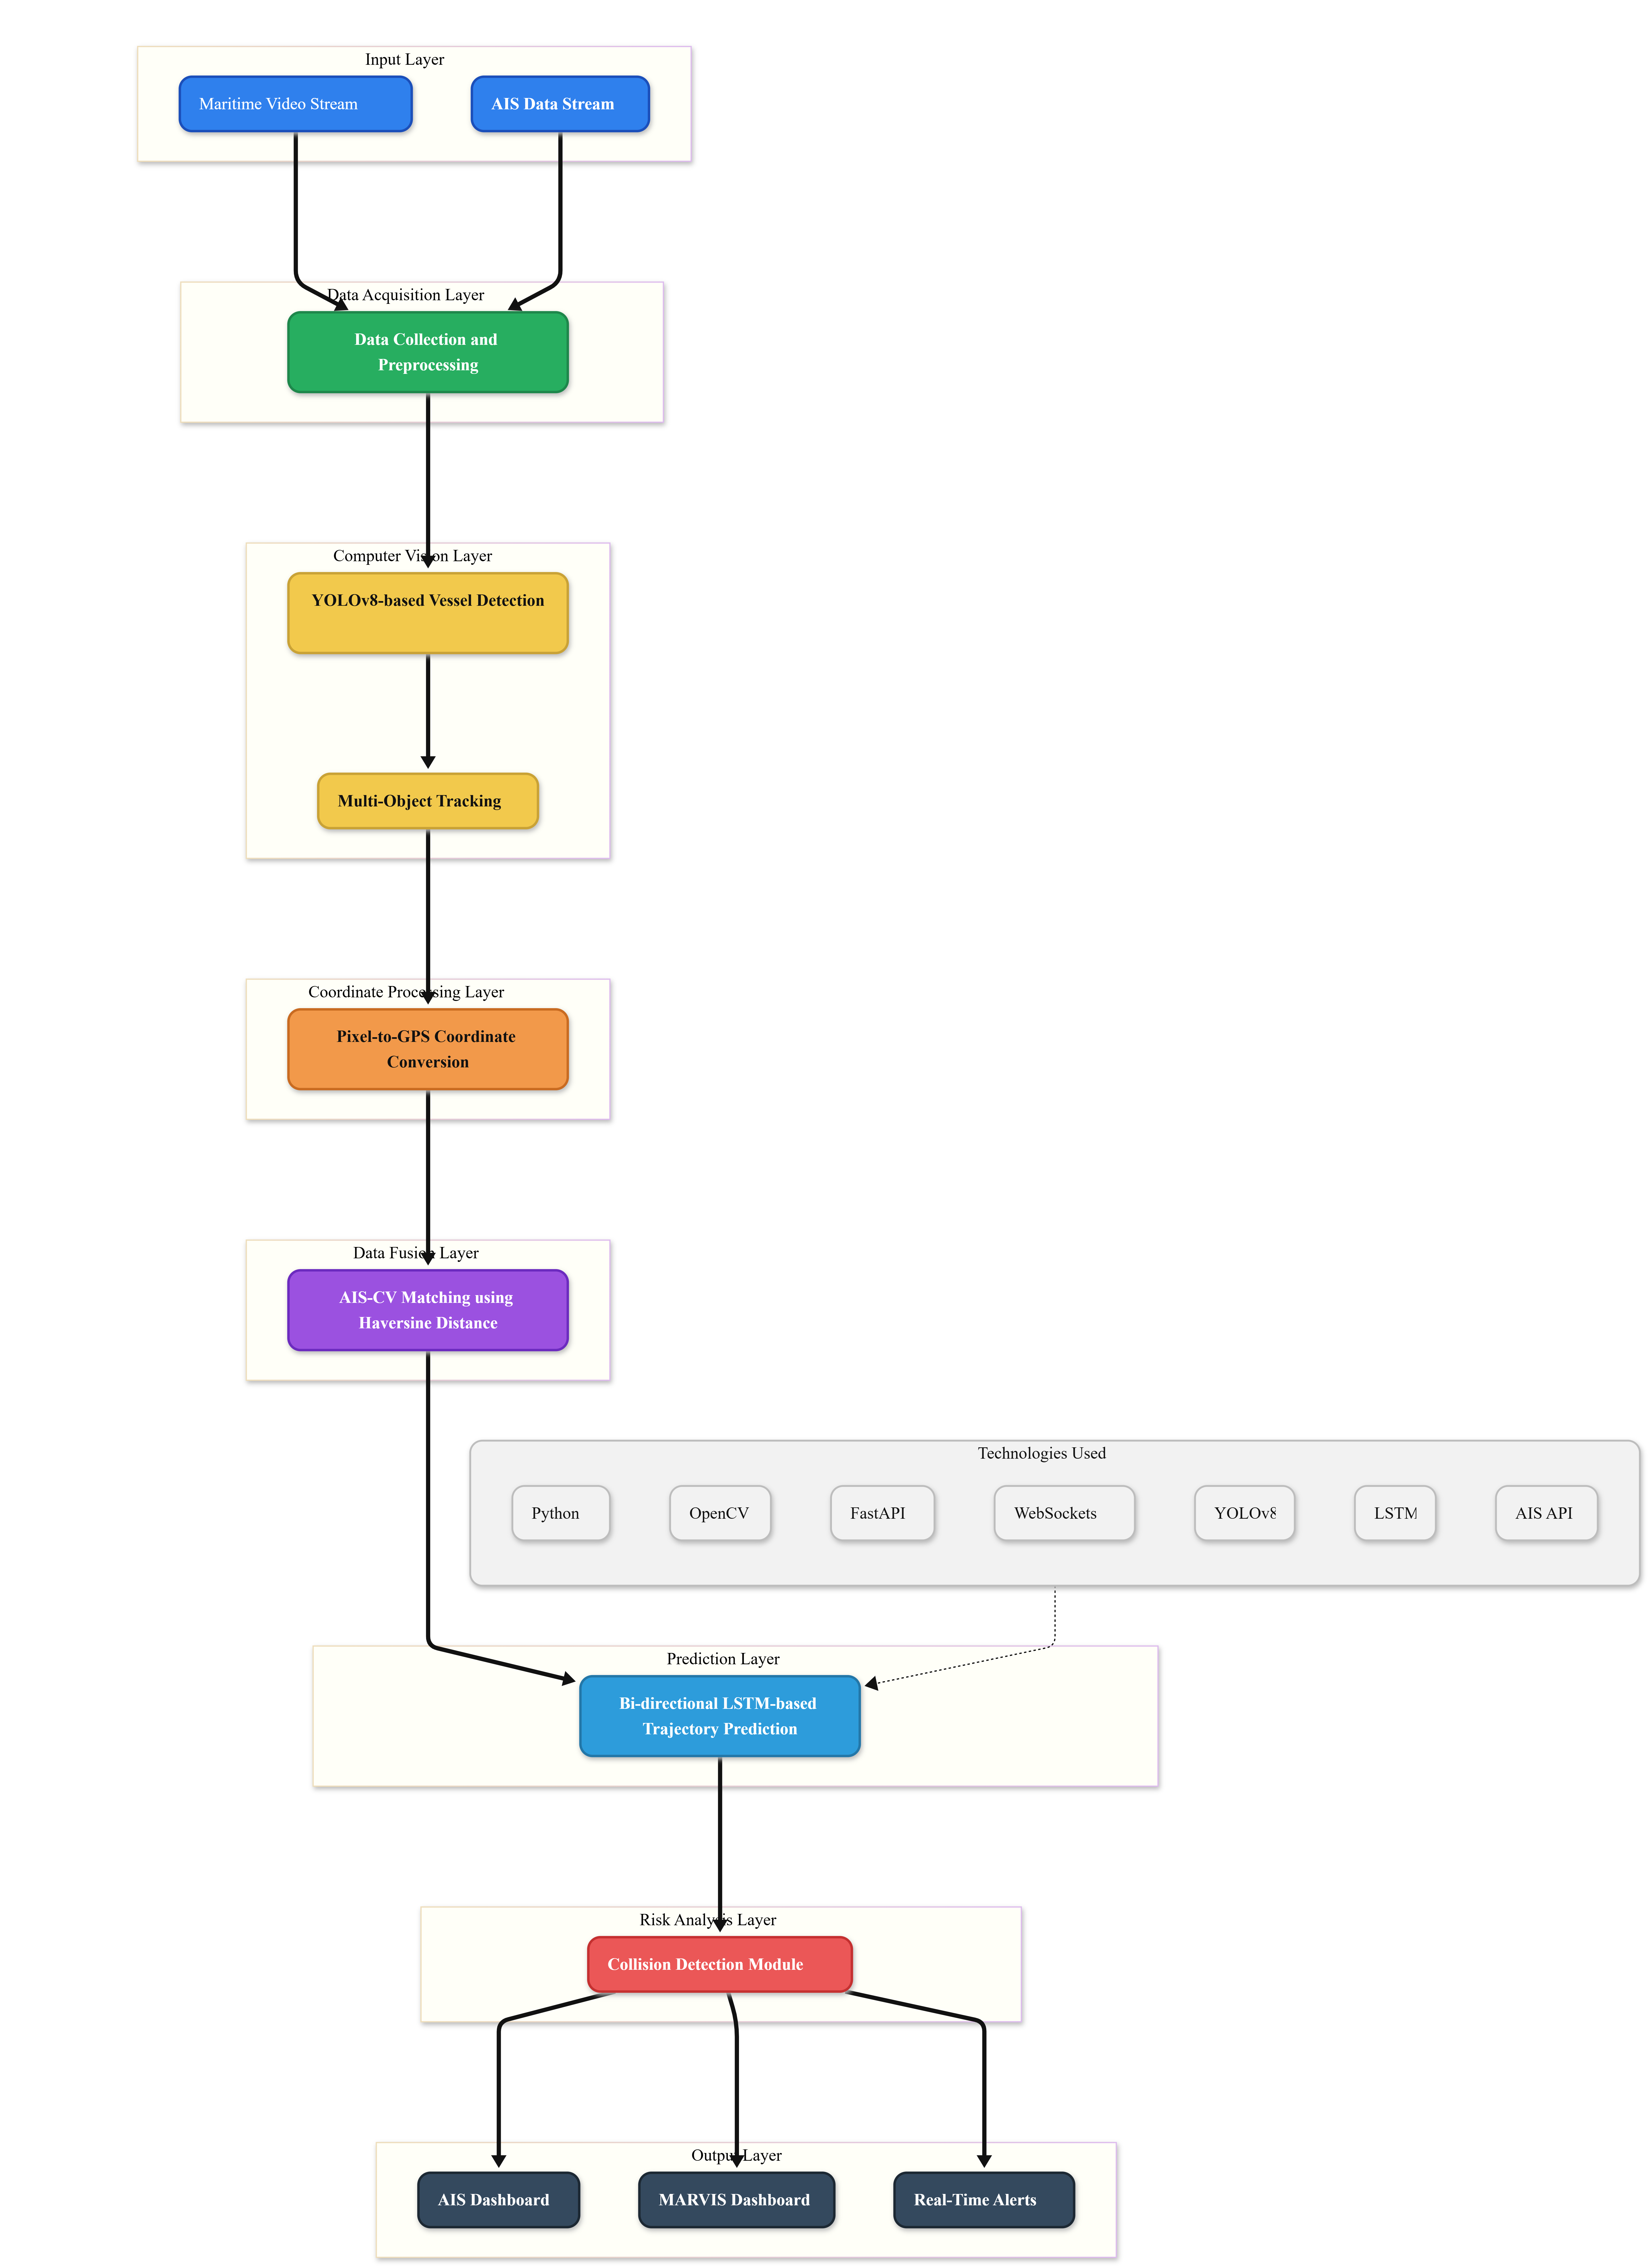
\includegraphics[width=0.95\textwidth]{Chapter3/Figures/system_architecture.png}
\caption{Overall Architecture of Proposed AI-Based Maritime Surveillance System}
\label{fig:architecture}
\end{figure}

\subsection{Development Methods}
Iterative development and modular design principles were employed.
\section{Architecture Strategies}
\subsection{Programming Language}
Python was selected for its extensive machine learning libraries including PyTorch and OpenCV.
\subsection{Future Plans}
Future versions aim to integrate radar data and expand to multi-camera spatial hand-offs.
\section{System Architecture}
\section{Data Flow Diagrams}

To map the exchange of information across external entities and internal modules, the system architecture was modeled using Data Flow Diagrams (DFDs).

\subsection{Context and Level-1 Diagrams}
The Level-0 Context Diagram (Figure~\ref{fig:dfd0}) provides a macro-level view of how users, camera feeds, and \gls{ais} streams interact with the central surveillance system.

\begin{figure}[!htbp]
\centering
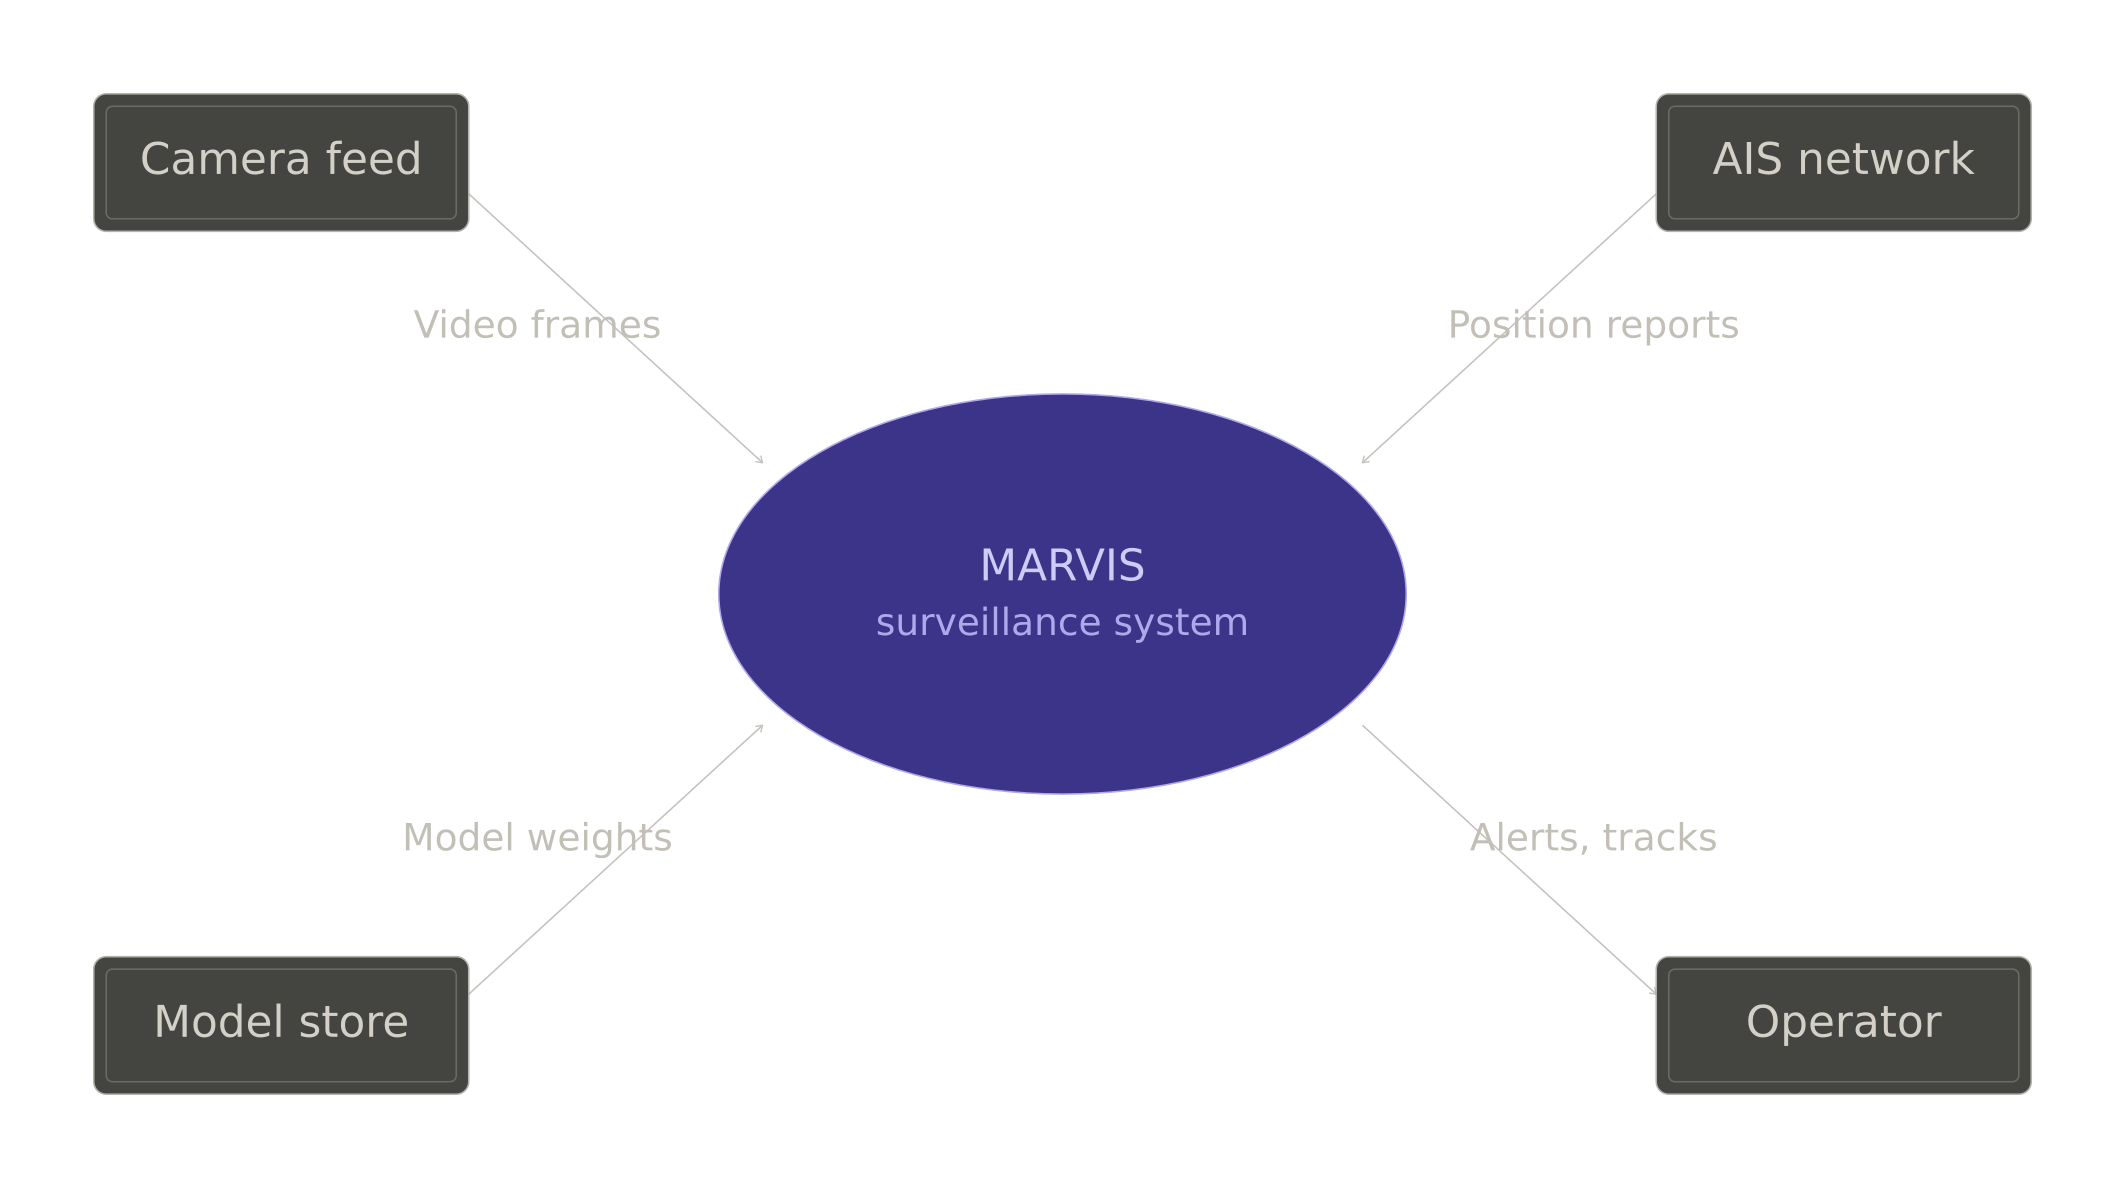
\includegraphics[width=0.95\textwidth]{Chapter3/Figures/dfd_level0_context.png}
\caption{Level-0 Context Diagram of Proposed Maritime Surveillance System}
\label{fig:dfd0}
\end{figure}

Expanding on this, the Level-1 DFD (Figure~\ref{fig:dfd1}) details the internal routing of this data. It illustrates how raw video frames are passed through detection and tracking, transformed into geographic coordinates, fused with telemetry, and finally routed into the \gls{bilstm} prediction and collision analysis modules before reaching the user dashboard.

\begin{figure}[!htbp]
\centering
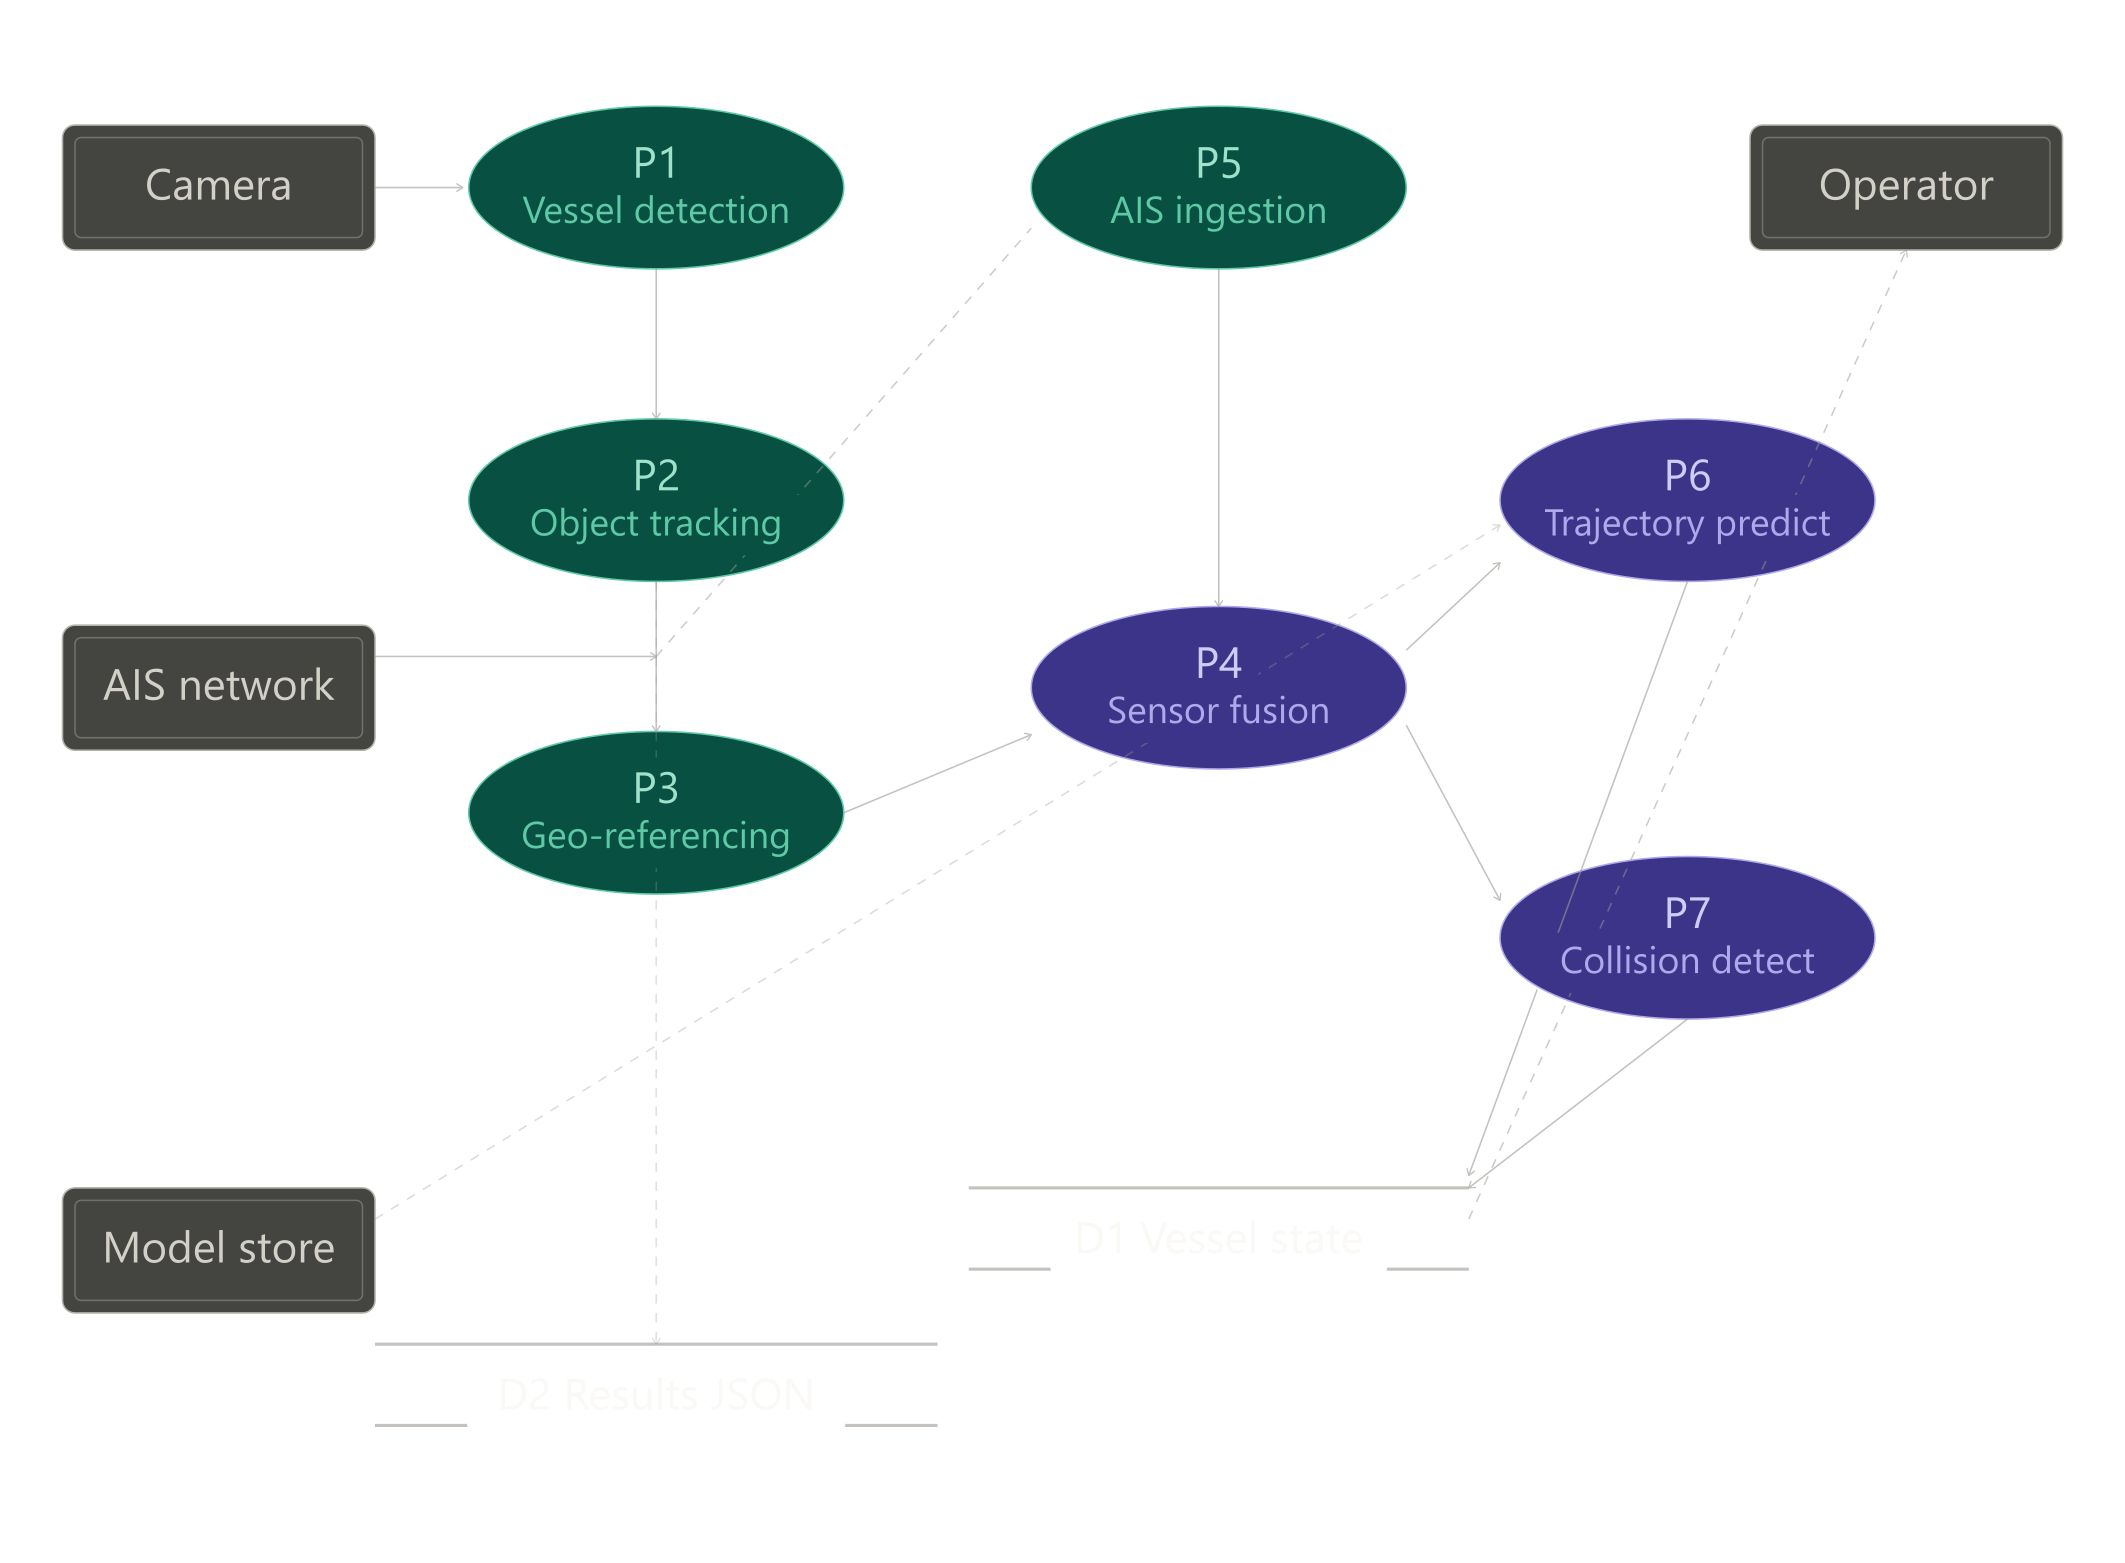
\includegraphics[width=0.95\textwidth]{Chapter3/Figures/dfd_level1_context.png}
\caption{Level-1 Data Flow Diagram of Proposed Maritime Surveillance System}
\label{fig:dfd1}
\end{figure}

\section{Summary}
This chapter presented the High Level Design including system architecture and data flow diagrams.
